\documentclass[12pt]{article}
\usepackage[spanish]{babel}
\usepackage[utf8x]{inputenc}
\usepackage{amsmath}
\usepackage{amsfonts}
\usepackage{graphicx}
\usepackage{float}
\usepackage[colorinlistoftodos]{todonotes}
\usepackage{mathtools}
\usepackage{tikz}
\usepackage{pgfplots}

\newcommand{\C}{\ensuremath{\mathbb{C}}} 
\newcommand{\R}{\ensuremath{\mathbb{R}}} 
\newcommand{\Z}{\ensuremath{\mathbb{Z}}} 
\newcommand{\N}{\ensuremath{\mathbb{N}}} 

\begin{document}

\begin{titlepage}

\newcommand{\HRule}{\rule{\linewidth}{0.5mm}} 

\center 
 

\textsc{\Large \bf{Universidad Nacional Autónoma de México}}\\[1.5cm] 
\textsc{\Large Facultad de Ciencias}\\[1.1cm] 


\includegraphics[scale=.08]{FacC}\\[1cm] 
\textsc{\Large Cálculo Diferencial e Integral II}\\[0.5cm] 
\textsc{\large Profesor: Raybel Andrés García Ancona}\\[0.2cm] 


\HRule \\[0.4cm]
{ \huge \bfseries Tarea 1}\\[0.2cm] 
\HRule \\[0.4cm]
 


\begin{minipage}{0.6\textwidth}
\begin{flushleft} \large
\emph{Autores:}\\
Andrés López González\\
Daniel Luis Pérez\\
Gael Ramses Lechuga Mireles\\
Lizeth Yamile Mendoza Acosta\\  
\end{flushleft}

\end{minipage}\\[2cm]




{\large \today}\\[2cm] 

\vfill 

\end{titlepage}

	\begin{enumerate}
		\item ¿Cuál es la función cuya derivada es la función
	\[ f(x) = \begin{dcases} x^2 \hspace{1cm} si\hspace{0.25cm} x<-2\\ 4 \hspace{1cm} si\hspace{0.25cm}-2\leq x\leq 2\\ x+2 \hspace{1cm} si \hspace{0.25cm}x>2 \end{dcases} \]
	? Haz la gráfica de las dos funciones.\\
			Usando la regla de exponenciales, se propone
			\[ F(x) = \begin{dcases} \frac{x^3}{3} \hspace{1cm} si\hspace{0.25cm} x<-2\\ 4x \hspace{1cm} si\hspace{0.25cm}-2\leq x\leq 2\\ \frac{x^2}{2}+2x \hspace{1cm} si \hspace{0.25cm}x>2 \end{dcases} \]
			Al comprobar la solución tenemos:
			\[ F'(x) = \begin{dcases} x^2 \hspace{1cm} si\hspace{0.25cm} x<-2\\ 4 \hspace{1cm} si\hspace{0.25cm}-2\leq x\leq 2\\ x+2 \hspace{1cm} si \hspace{0.25cm}x>2 \end{dcases} \]
			Con lo cual se puede concluir que la función propuesta al derivarse nos da la función dada. \\
			La gráfica de f(x) es\\
		\begin{center}			
		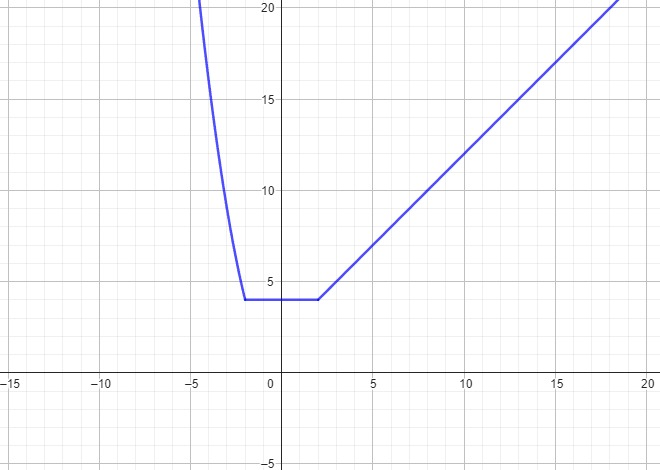
\includegraphics[scale=.6]{Graf1}\\
		\end{center}
			Mientras que F(x):\\
		\begin{center}
		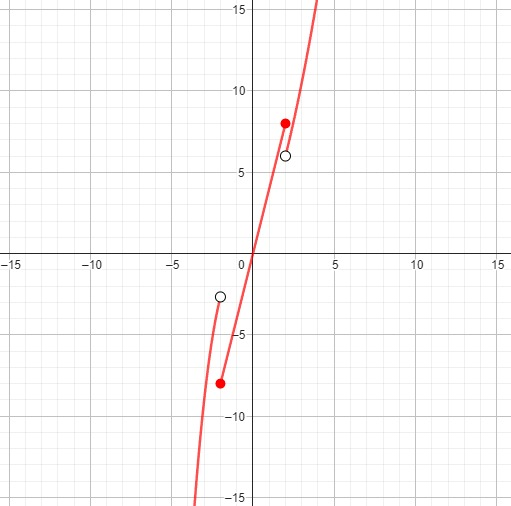
\includegraphics[scale=.6]{Graf2}\\
		\end{center}
		\item Encuentra una función cuya derivada es:
		\begin{enumerate}
			\item $3 sin(3x)$\\	
			Al considerar que la derivada de la función coseno nos devuelve un signo menos, se propone la función:\\
			 \[F(x)= -cos(3x)\]
			Lo cual, al derivarse, nos daría: 
			\[F'(x)=-(3)(-sen(3x))=3sin(3x)\]
			\item $x cos(x^2+1)$\\
			Recordando la regla de la cadena, se propone la función:
			\[F(x)=sen(x^2+1) \]
			\[ \Rightarrow F'(x)=2x(cos(x^2+1))\]
			Sobra un $2$, por lo que la función que al derivarse nos da la función deseada es:
			\[F(x)= \frac{1}{2}sen(x^2+1) \]
			\item $sin^3(x)cos(x)$\\
			Considerando la regla de la cadena y de los exponentes, se propone la función
			\[F(x)=\frac{1}{4}sen^4(x)\]
			Al derivar obtenemos:
			\[F'(x)=\frac{1}{4}4sen^3(x)cos(x)=sen^3(x)cos(x)\]
			\item $sin(x+1)cos(x+1)$\\
			Se propone la función\[F(x)=\frac{1}{2}sen^2(x+1)\]
			Derivando \[F'(x)=\frac{1}{2}2sen(x+1)cos(x+1)=sen(x+1)cos(x+1)])\]
			\item $tan^2(x)$\\
			Usando identidades trigonométricas obtenemos
			\[tan^2(x)=sec^2(x)-1 \]
			Entonces, usando la tabla básica de integrales, se propone
			\[F(x)=tan(x)-x\]
			Lo cual, al derivarse
			\[F'(x)=sec^2(x)-1=tan^2(x)\]
			\item $\dfrac{1}{\sqrt{4-x^2}}$\\
			La única función conocida que da una raíz con un polinomio cuadrático sin término lineal y que esté dentro de una raíz, son las inversas trigonométricas, con lo cual, buscándo darle la forma conocida a la ecuación dada, tenemos:
			\[\dfrac{1}{\sqrt{4-x^2}}=\dfrac{1}{\sqrt{4(1-\frac{x^2}{4})}}=\dfrac{1}{2\sqrt{1-(\frac{x}{2})^2}}\]
			Y a partir de la tabla básica de integrales, se propone
			\[F(x)=arcsen\bigl(\frac{x}{2}\bigr)\]
			Lo que al derivarse
			\[F'(x)=\frac{1}{2}\Bigl(\dfrac{1}{\sqrt{1-(\frac{x}{2})^2}}\Bigr)=\dfrac{1}{\sqrt{4-x^2}}\]
			\item $\dfrac{1}{\sqrt{25-x^2}}$\\
			Nuevamente, se busca dar una forma conocida a la función dada, entonces:
			\[\dfrac{1}{\sqrt{25-x^2}}=\dfrac{1}{\sqrt{25(1-\frac{x^2}{25})}}=\dfrac{1}{5\sqrt{1-(\frac{x}{5})^2}}\]
			Usando la tabla básica de integrales, tenemos
			\[F(x)=arcsen(\frac{x}{5})\]
			Derivando
			\[F'(x)=\frac{1}{5}\Bigl(\dfrac{1}{\sqrt{1-(\frac{x}{5})^2}}\Bigr)=\dfrac{1}{\sqrt{25-x^2}}\]
			\item $\dfrac{1}{x^2+2x+2}$\\
			En este caso, al tener un denominador completamente positivo con un témrino cuadrático, se busca darle la forma de la derivada del arcotangente, entonces
			\[\dfrac{1}{x^2+2x+2}=\dfrac{1}{x^2+2x+1-1}\dfrac{1}{(x+1)^2+1}\]
			Ahora bien, por la tabla básica de integrales, se propone
			\[F(x)=arctan(x+1)\]
			\item $\dfrac{x}{1+x^4}$\\
			Nuevamente, buscando darle la forma de la derivada del arcotangente y recordando que sería posible justificar la x en el numerador por la regla de la cadena:
			\[\dfrac{x}{1+x^4}=\dfrac{x}{1+(x^2)^2}\]
			Se propone
			\[F(x)=\frac{1}{2}arctan(x^2)\]
			Aplicando la regla de la cadena al derivar
			\[F'(x)=\frac{1}{2}(2x)\dfrac{1}{1+(x^2)^2}=\dfrac{x}{1+x^4}\]
			\item $\dfrac{1}{\sqrt{4x-x^2}}$\\
			Queremos encontrar una forma conocida en la función dada, por lo cual, se buscará hacer a parecer un solo término cuadrático en el denominador y desaparecer el término lineal.
			\[\dfrac{1}{\sqrt{4x-x^2}}=\dfrac{1}{\sqrt{(-1)(x^2-4x+4-4)}}=\dfrac{1}{\sqrt{(-1)((x-2)^2-4)}}\]
			\[=\dfrac{1}{\sqrt{4-(x-2)^2}}=\dfrac{1}{\sqrt{4(1-\frac{(x-2)^2}{4})}}=\dfrac{1}{2\sqrt{1-(\frac{x-2}{2})^2}}\]
			Por lo que se propone
			\[F(x)=arcsen(\frac{x-2}{2})\]
			Que al derivarse
			\[F'(x)=\dfrac{1}{2\sqrt{1-(\frac{x-2}{2})^2}}=\dfrac{1}{\sqrt{4x-x^2}}\]
		\end{enumerate}
		\item Obtener las funciones cuyas derivadas son las siguientes funciones\\
		Dado que el ejercicio plantea más de una función que al derivarse nos arroje la función indicada, debemos considerar todas aquellas funciones que disten unas de las otras por una constante real. 
		\begin{enumerate}
			\item$x^{-4}$\\
			En este caso, se propone: 
			\[F(x)=\dfrac{-x^{-3}}{3}+c \hspace{0.15cm},\hspace{0.20cm} c\in\R\]
			Al derivar
			\[F'(x)=-(-3)\dfrac{x^{-4}}{3}=x^{-4} \]
			\item$x^{\frac{7}{2}}$\\
			Se propone a la función
			\[F(x)=-\frac{2}{5}x^{-\frac{5}{2}}+c \hspace{0.15cm},\hspace{0.20cm} c\in\R\]
			Al derivarse
			\[F'(x)=-\frac{2}{5}(\frac{-5}{2})x^{-\frac{7}{2}}=x^{-\frac{7}{2}}\]
			\item$x^{-5}+x^{-2}+1$\\
			Se propone a la función
			\[F(x)=-\dfrac{x^{-4}}{4}+\dfrac{-x^{-1}}{1}+x+c \hspace{0.15cm},\hspace{0.20cm} c\in\R\]
			Derivando
			\[F'(x)=\frac{-1}{4}(-4)x^{-5}+x^{-2}+1=x^{-5}+x^{-2}+1\]
			\item$3x^{-3}+2x^{-2}$\\
			Se propone la función 
			\[F(x)=-\frac{3}{2}x^{-2}-2x^{-1}+c \hspace{0.15cm},\hspace{0.20cm} c\in\R\]
			Al derivarse
			\[F'(x)=-\frac{3}{2}(-2)x^{-3}-2(-1)x^{-2}=3x^{-3}+2x^{-2}\]
			\item$x^{-7}+x^3-4$\\
			Se propone 
			\[F(x)=-\dfrac{x^{-6}}{6}+\dfrac{x^{4}}{4}-4x+c \hspace{0.15cm},\hspace{0.20cm} c\in\R\]
			Ya que al derivarse
			\[F'(x)=\frac{-1}{6}(-6)x^{-7}+\frac{1}{4}(4)x^3-4=x^{-7}+x^3-4\]			
			\item$2x(x^2+1)$\\
			Por la regla de la cadena, se propone
			\[F(x)=\dfrac{(x^2+1)^2}{2}+c \hspace{0.15cm},\hspace{0.20cm} c\in\R\]
			Comprobando la propuesta, tenemos
			\[F'(x)=\dfrac{2(x^2+1)}{2}2x=2x(x^2+1)\]
			\item$(x^2+1)^2$\\
			Reescribiendo la expresión
			\[(x^2+1)^2=x^4+2x^2+1\]
			Recordando la regla de los exponentes, tenemos:
			\[F(x)=\dfrac{x^5}{5}+\frac{2}{3}x^3+x+c \hspace{0.15cm},\hspace{0.20cm} c\in\R\]
			Al derivar:
			\[F'(x)=\frac{5}{5}x^4+\frac{6}{3}x^2+1=x^4+2x^2+1=(x^2+1)^2\]
			\item$\dfrac{3x}{(x^2+1)^2}$\\
			Recordando la regla de la cadena y la tabla básica de integrales:
			\[F(x)=\dfrac{-3}{2(x^2+1)}+c \hspace{0.15cm},\hspace{0.20cm} c\in\R\]
			Lo cual, al derivarse:
			\[F'(x)=-\frac{3}{2}\Bigl(\dfrac{-1}{(x^2+1)^2}\Bigr)2x=\dfrac{3x}{(x^2+1)^2}\]
			\item$(x^3+x^2+1)^3(3x^2+2x)$\\
			Se puede observar que un término es muy cercano a la derivada del otro, con lo que se propone la función
			\[F(x)=\frac{1}{4}(x^3+x^2+1)^4+c \hspace{0.15cm},\hspace{0.20cm} c\in\R\]
			Derivando
			\[F'(x)=\frac{1}{4}(3x^2+2x)4(x^3+x^2+1)^3=(x^3+x^2+1)^3(3x^2+2x)\]
			\item$\dfrac{2x+5}{\sqrt{x^2+5x+1}}$\\
			Sabemos que
			\[\dfrac{2x+5}{\sqrt{x^2+5x+1}}=(2x+5)(x^2+5x+1)^{-\frac{1}{2}}\]
			Entonces se propone la función
			\[F(x)=2(x^2+5x+1)^\frac{1}{2}+c \hspace{0.15cm},\hspace{0.20cm} c\in\R\]
			Derivando
			\[F'(x)=2\Bigl(\frac{1}{2}(x^2+5x+1)^{-\frac{1}{2}}(2x+5)\Bigr)=(2x+5)(x^2+5x+1)^{-\frac{1}{2}}\]
			\[=\dfrac{2x+5}{\sqrt{x^2+5x+1}}\]
			\item$(x^2-2x+7)^{-2}(x-1)$\\
			Por regla de la cadena
			\[F(x)=\frac{-1}{2}(x^2-2x+7)^{-1}+c \hspace{0.15cm},\hspace{0.20cm} c\in\R\]
			\[\Rightarrow F'(x)=-\frac{-1}{2}(x^2-2x+7)^{-2}(2x-2)=\frac{1}{2}2(x-1)(x^2-2x+7)^{-2}\]
			\[=(x^2-2x+7)^{-2}(x-1)\]
			\item$x^2\sqrt{x^3+1}$\\
			Por regla de la cadena
			\[F(x)=\frac{2}{3}(x^3+1)^{\frac{3}{2}}+c \hspace{0.15cm},\hspace{0.20cm} c\in\R\]
			\[\Rightarrow F'(x)=\frac{2}{3}\frac{3}{2}(x^3+1)^{\frac{1}{2}}(3x^2)=3x^2\sqrt{x^3+1}\]
			Sobra un factor de 3
			\[\Rightarrow F(x)=\frac{2}{9}(x^3+1)^{\frac{3}{2}}+c \hspace{0.15cm},\hspace{0.20cm} c\in\R\]
			\item$(x+a)^n$\\
			Por regla de exponentes
			\[F(x)=\dfrac{(x+a)^{n+1}}{n+1}+c \hspace{0.15cm},\hspace{0.20cm} c\in\R\]
			\[\Rightarrow F'(x)=\dfrac{n+1}{n+1}(x+a)^{n+1-1}=(x+a)^n\]
			\item$x(x^2+a)^n$\\
			Por regla de la cadena se supone
			\[F(x)=\dfrac{(x^2+a)^{n+1}}{2(n+1)}+c \hspace{0.15cm},\hspace{0.20cm} c\in\R\]
			\[\Rightarrow F'(x)=\dfrac{n+1}{2(n+1)}(x^2+1)^n2x=x(x^2+a)^n \]
		\end{enumerate}						
	\end{enumerate}
	
\end{document}